\chapter{Basics of Deep Learning} \label{chap:basics-of-dl}

Deep learning is an area of machine learning that uses Artificial Neural Networks \parencite{mcculloch1943logical} and has been applied to a wide variety of tasks such as image classification, object recognition, activity recognition, 3D depth estimation and various natural language processing (NLP) tasks. In stark contrast to classical machine learning approach of designing manual feature extraction methods, deep learning focuses on making algorithms that can naturally learn to extract the relevant features.

\section{Deep Feedforward Networks} \label{sec:feed-forward-nets}

Deep feedforward networks, also called feedforward networks, or \textbf{multilayer perceptrons} (MLPs), are the essential deep learning models. The goal of a feedforward network is to approximate some ideal function \(f^\star\). 
For example, a classifier \(y = f^\star(\symbfit{x})\) is a mapping between input $\symbfit{x}$ to a category $y$. A feedforward network has the capability to learn this mapping \(\symbfit{y} = f(\symbfit{x}; \symbfit{\theta})\) where $\symbfit{\theta}$ is a set of learned parameters that result in the best function approximation. In other words, neural networks (deep or otherwise) are function approximators.

Such models are called \textbf{feedforward} as the information flows through the function which evaluates $\symbfit{x}$ and outputs $\symbfit{y}$. The process of passing the input $\symbfit{x}$ through the function and through intermediate computations is known as the \textbf{forward pass}. We then use a \textbf{loss function} to measure the difference between $f^\star$ and $f$ - that is, the difference between the ideal mapping $f^\star$ and estimated mapping $f$. The parameters of the network $\symbfit{\theta}$ are updated in a \textbf{backward pass} based on some optimisation criteria, given the guidance of the loss function. 

% \includesvg{./assets/mlp.svg}
\begin{figure}
    \centering
    \captionsetup{justification=centering}
    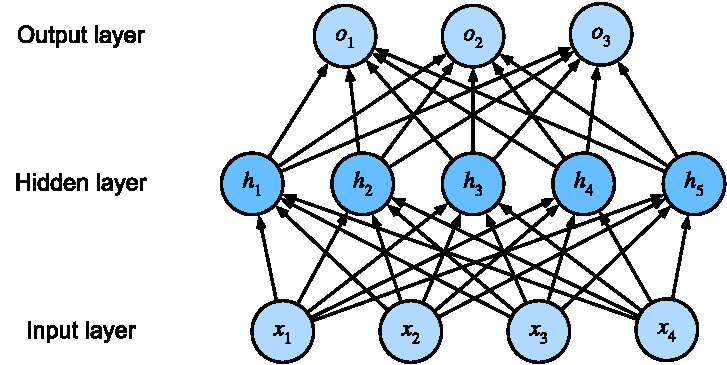
\includegraphics[scale=0.9]{chapters/assets/mlp.pdf}
    \caption{An MLP with hidden layer consisting of $5$ hidden units. Image borrowed from D2L book \parencite{zhang2021dive}.}
    \label{fig:mlp}
\end{figure}

Feedforward neural networks are called \textit{networks} as they are typically compositions of many different functions. The model is associated with a directed acyclic graph describing how the functions are composed together.
For example, we may have three functions \(f^{(1)}, f^{(2)}\) and $f^{(3)}$ connected in a chain, to form \(f = f^{(1)} \circ f^{(2)} \circ f^{(3)}\). 
Chain structures like these are quite commonly used structures of neural networks. Here, $f^{(1)}$ is the \textbf{first layer}, $f^{(2)}$ is the \textbf{second layer} and so on. 
The final layer is referred to as the \textbf{output layer}, in this small example, $f^{(3)}$ is the output layer. The training data or training strategy determines what the output layer must produce for each given input $\symbfit{x}$.
Intermediate layers like $f^{(2)}$ which do not directly produce the output $\symbfit{y}$ are called \textbf{hidden layers}.

Each hidden layer of the network is typically vector valued. The dimensionality of these hidden layers determines the \textbf{width} of the model. Each element in the vector plays a role analogous to a neuron. Instead of reasoning about a layer as a vector-to-vector function, we can also think of the layer as consisting of many \textbf{units} that act in parallel \parencite{Pinker1988}, each representing a vector-to-scalar function. 
\Cref{fig:mlp} shows a small MLP with a single hidden layer. Each of the nodes in \cref{fig:mlp} represents a value of a vector, this implies that the input $\symbfit{x}$ has a dimensionality of $4$, hidden layer (intermediate values) has a dimensionality of $5$ and the output has a dimensionality of $3$.

Now we must choose the form of our model, $f(\symbfit{x};\symbfit{\theta})$. Let us choose a linear model parametrised by $\symbfit{\theta}$ consisting of $\symbfit{w}$ and $b$, where $\symbfit{w}$ provides the weights and $b$ provides the biases (or intercepts):

\begin{equation}\label{eqn:linear-model}
    f(\symbfit{x}; \symbfit{\theta}) = f(\symbfit{x} ; \symbfit{w}, b)=\symbfit{x}^{\top} \symbfit{w} + b.
\end{equation}

For the model in \cref{fig:mlp} whose hidden layer has $\symbfit{h}$ units, that are computed by a function \(f^{(1)}(\symbfit{x}; \symbfit{W}, \symbfit{c})\) which is linear similar to the form of \cref{eqn:linear-model}. The values of these hidden units are then used as the input for the second layer, which is also the output layer of the network. The output layer is also a linear function applied to $\symbfit{h}$ rather on to $\symbfit{x}$.
The network now has two functions chained together \(\symbfit{h} = f^{(1)}(\symbfit{x}; \symbfit{W}, \symbfit{c})\) and \(y = f(\symbfit{h} ; \symbfit{w}, b)\), with the complete model being $f(\symbfit{x} ; \symbfit{W}, \symbfit{c}, \symbfit{w}, b)=f^{(2)}\left(f^{(1)}(\symbfit{x})\right)$. 

Unfortunately, the complete model $f$ is linear function of its input as we have chosen both $f^{(1)}$ and $f^{(2)}$ to be linear. 
However, not all data spaces are linear. More often than not they are of non-linear nature, accordingly we must introduce a non-linear function to describe the data and its features.
Most neural networks do so using an affine transformation controlled by learned parameters (such as $\symbfit{\theta}$), followed by a fixed non-linear function called an \textbf{activation function}.

\section{Activation Functions} \label{sec:activation-functions}

Activation functions decide whether or not a neuron (node in \cref{fig:mlp}) should be activated 


\section{Universal Approximation Theory}\label{sec:uat}

MLPs are of extreme importance in deep learning, as they form the basis of many applications and advanced neural architectures. To do this, MLPs and neural networks in general, must be able to approximate a wide range of functions - given enough input data to learn from. Neural networks started out as way to mimic the neural structure of the brain \parencite{mcculloch1943logical}, and as we know our brain is capable of complex statistical analysis among other things. As such, a worthwhile question to be asked here is, \textit{just how powerful can a deep neural network be?}.
Fortunately for us, this question has been answered several times in the context of MLPs and radial basis functions (RBF) \parencite{Cybenko1989, Micchelli1986, Hornik1991}. These works suggest that even with a single hidden layer, given enough nodes, and the right set of parameters $\symbfit{\theta}$, we can model any function. Even though neural networks are capable of expressing arbitrary continuous functions it may not be easy to learn the function and its parameters.